\documentclass{beamer}
\usepackage{framed}
\usepackage{graphicx}

\begin{document}
\section{Integer Programming}
\subsection{Canonical Form}
%================================================ %
\begin{frame}
	\frametitle{Canonical Form}
\begin{figure}
\centering
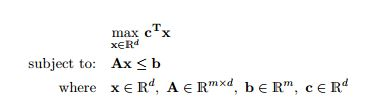
\includegraphics[width=0.7\linewidth]{canonical}
\caption{}
\label{fig:canonical}
\end{figure}
The polyhedron P, our feasible region, is defined by the set of inequalities Ax ≤ b. In two
dimensions, i.e. if d = 2, this problem can be represented and solved graphically. The idea
is to represent the cost vector c as a level set in the plane. Then, moving this level set
towards the highest possible value so that still intersects our feasible region, i.e. the polyhedron
P defined by A, yields the optimal solution.
\end{frame}

%================================================ %
\subsection{LP Divisibility}
\begin{frame}
\frametitle{Divisibility}	
\begin{itemize}
\item Divisibility is one of the conventional LP assumptions.
\item Divisibility allowed us to consider activities in fractions: We could produce 7.8 units of a product,
buy 12500.33 liters of oil, hire 12.123 people for full time, etc. 
\item Divisibility assumption is very defensible at
times but not always. 
\item We can easily buy 12500.33 liters of oil but can not employ 12.123 people. 
\end{itemize}
\end{frame}

%================================================= %
\begin{frame}
\frametitle{Divisibility}
\begin{itemize}
\item Clearly
some activities cannot be done in fractions and must be specified in integers for implementation.
\item As soon as
 some of the activities are set to be integers, we are in \textbf{Integer Programming} domain. 
 \item Formally, in an integer
 program some decision variables are forced to be integers.
\end{itemize}
\end{frame}
%================================================== %
\subsection{Lattice Point}
\begin{frame}
	\begin{figure}
\centering
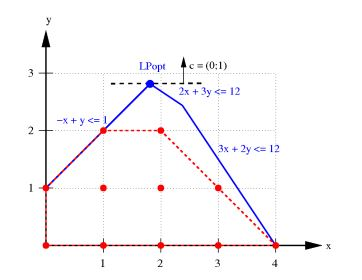
\includegraphics[width=0.7\linewidth]{LatticePoints}
\caption{}
\label{fig:LatticePoints}
\end{figure}

\end{frame}
\subsection{Example of IP Problem}
\begin{frame}
\frametitle{IP Example:  Tables and Chairs}
\begin{itemize}
	\item Suppose we consider producing chairs and tables using only 21 $m^2$ of
	wood. Each chair (table) requires 6 (7) $m^2$ of wood. 
	\item Each chair is sold at $\$12$ (×10) and each table is sold
	at $\$13$ ($\times 10$). 
	\item Let C and T denote the number of tables and chairs produced. 
	\item The IP formulation below
	maximizes the revenue:
\end{itemize}
\end{frame}
%======================================================================== %
\begin{frame}
\frametitle{IP Example:  Tables and Chairs}
\begin{figure}
\centering
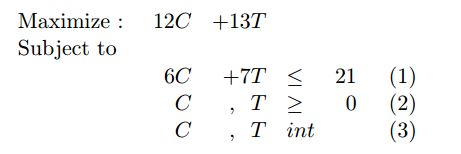
\includegraphics[width=0.7\linewidth]{IPintro1}
\end{figure}

\end{frame}
%============================================================================== %
\begin{frame}
\frametitle{IP Example:  Tables and Chairs}
\begin{figure}
\centering
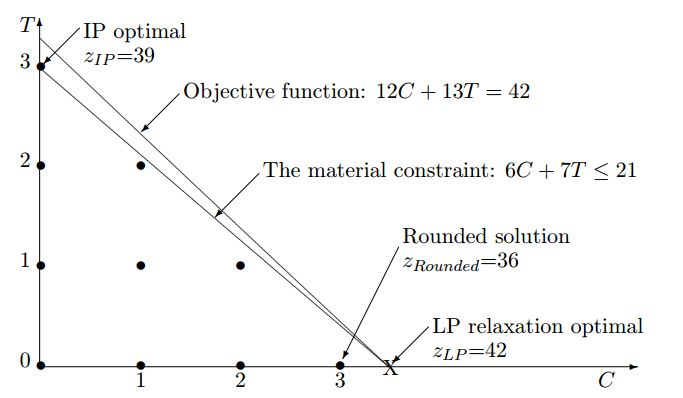
\includegraphics[width=0.7\linewidth]{IPintro2}
\caption{}
\label{fig:IPintro2}
\end{figure}
\end{frame}
%================================================ %
\subsection{LP Relaxation}
\begin{frame}
\frametitle{LP Relaxation}
\begin{itemize}
\item 
Solving an IP can be as straightforward as solving the associated LP
and rounding the solution, but only in some cases. (i.e. by coincidence rather than by definition)
\item To understand what can wrong with this approach, we will first solve the IP
removing constraint (3) and round down (why not to round up?) the optimal values of C and T to satisfy
(3). 
\item When the integer constraints are removed from an IP formulation, we obtain an LP formulation. This
LP formulation is called the \textbf{LP relaxation}.
\end{itemize}
\end{frame}
%======================================================= %
\begin{frame}
	\frametitle{LP Relaxation}
	\begin{itemize}
\item LP solution is (7/2,0) and is not integer so we round it down to (3,0). 
\item The objective value at (3,0) is
36. 
\item The optimal solution to IP is (0,3) with the objective value 39. 
\item 3 units of difference between objective
value of the IP optimal and the rounded solution can be significantly higher in more complex problems.
\item As
a summary we cannot use rounded solutions of LP relaxations.
	\end{itemize}
\end{frame}
%======================================================= %
\begin{frame}
\frametitle{LP Relaxation}
Given an integer program (IP), there is an associated Hnear program (LR)
called the linear relaxation. It is formed by dropping (relaxing) the integrality
restrictions. Since (LR) is less constrained than (IP), the following are immediate:
\begin{itemize}
\item[1] If (IP) is a minimization problem, the optimal objective value of (LR) is
less than or equal to the optimal objective value of (IP).
\item[2] If (IP) is a maximization problem, the optimal objective value of (LR) is
greater than or equal to the optimal objective value of (IP),
\item[3] If (LR) is infeasible, then so is (IP).
\item[4] If all the variables in an optimal solution of (LR) are integer-valued, then
that solution is optimal for (IP) too.
\end{itemize}
\end{frame}
\begin{frame} 
\begin{itemize}
\item[5] If the objective function coefficients are integer-valued, then for minimization
	problems, the optimal objective value of (IP) is greater than
	or equal to the ceiling of the optimal objective value of (LR). For maximization
	problems, the optimal objective value of (IP) is less than or
	equal to the floor of the optimal objective value of (LR). 
\end{itemize}
\end{frame}
%=============== %
\subsection{Solution Techniques}
\begin{frame}
\begin{itemize}
\item For simple problems one
	can evaluate all the integer solutions in the feasible region and pick the best. 
\item However, for real problems
	this approach will take practically infinite amount of time. 
\item The solution procedures for IP’s are still under
	development. 
\item Two approaches are common: Branch and Bound technique, and Cutting planes. 
\item These
	techniques are outside the scope of our discussion.
\end{itemize}

\end{frame}
%======================================================= %
\subsection{Binary Integer Problems}
\begin{frame}
\frametitle{Zero-One Integer Problems}
	Zero-one linear programming involves problems in which the variables are restricted to be either 0 or 1. Note that any bounded integer variable can be expressed as a combination of binary variables.
\end{frame}
%======================================= %

\subsection{Capital Budgeting}
\begin{frame}
\frametitle{Capital Budgeting}
\Large
\begin{itemize}
\item	A firm has $n$ projects that it would like to undertake but because of budget limitations not all can be
	selected. 
\item In particular project $j$ is expected to produce a revenue of $c_j$ but requires an investment of $a_{ij}$ in the time period i for $i \in 1 \ldots m$. 
\item The capital available in time period  is $b_i$ . 
\end{itemize}
\end{frame}
%===================================== %
\begin{frame}
	\frametitle{Capital Budgeting}
	\Large
	\begin{itemize}
		\item The problem of maximising revenue subject to i
	the budget constraints can be formulated as follows: let $x_j$ = 0 or 1 correspond to not proceeding or 	respectively proceeding with project j then we have to
\end{itemize}
\begin{figure}
\centering
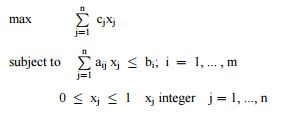
\includegraphics[width=0.7\linewidth]{capitalbudgeting}
\end{figure}

\end{frame}
%======================================================= %
\subsection{Knapsack Problems}
% - https://www.utdallas.edu/~metin/Or6302/Notes/integer.pdf
%- http://www.geeksforgeeks.org/dynamic-programming-set-10-0-1-knapsack-problem/

\begin{frame}
\begin{figure}
\centering
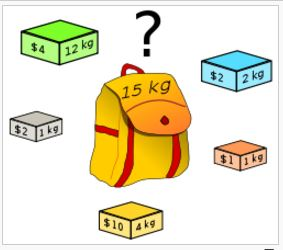
\includegraphics[width=0.7\linewidth]{knapsack}
\caption{}
\label{fig:knapsack}
\end{figure}
\end{frame}
%======================================================= %
\begin{frame}
	\frametitle{The Knapsack Problem}
\Large
\begin{itemize}
\item The knapsack problem or rucksack problem is a problem in combinatorial optimization: Given a set of items, each with a weight and a value, determine the number of each item to include in a collection so that the total weight is less than or equal to a given limit and the total value is as large as possible.
\end{itemize}
	
\end{frame}
\begin{frame}
	The most common problem being solved is the 0-1 knapsack problem, which restricts the number xi of copies of each kind of item to zero or one. Given a set of n items numbered from 1 up to n, each with a weight wi and a value vi, along with a maximum weight capacity W,
\begin{figure}
\centering
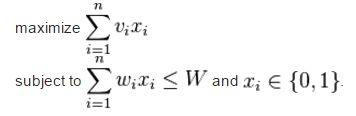
\includegraphics[width=0.7\linewidth]{01knapsack}
\caption{}
\label{fig:01knapsack}
\end{figure}
\end{frame}
\begin{frame}
	\frametitle{Knapsack Problems}
	\Large
	Here xi represents the number of instances of item i to include in the knapsack. Informally, the problem is to maximize the sum of the values of the items in the knapsack so that the sum of the weights is less than or equal to the knapsack's capacity.
\end{frame}
\begin{frame}
	\frametitle{Knapsack Problems}
	\Large
\begin{itemize}
\item Remark: The 0-1 knapsack problems is an optimization problem.
	\item Brute force: Try all $2^n$ possible subsets (Recall definition of Power Set)
	.
\item	Question: Any solution better than the brute-force?
\end{itemize}
\end{frame}
\begin{frame}
	\frametitle{Knapsack Problems}
\Large
The bounded knapsack problem (BKP) removes the restriction that there is only one of each item, but restricts the number $x_i$ of copies of each kind of item to an integer value $c_i$:
\begin{figure}
\centering
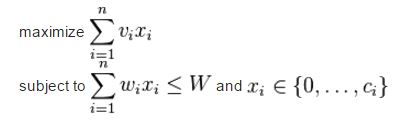
\includegraphics[width=0.7\linewidth]{boundedknapsack}
\caption{}
\label{fig:boundedknapsack}
\end{figure}
\end{frame}
%================================================= %
\begin{frame}
	\frametitle{Knapsack Problems}
	\Large
The unbounded knapsack problem (UKP) places no upper bound on the number of copies of each kind of item and can be formulated as above except for that the only restriction on $x_i$ is that it is a non-negative integer.
	\begin{figure}
\centering
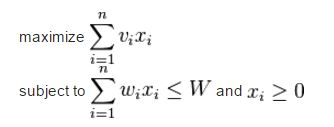
\includegraphics[width=0.7\linewidth]{unboundedknapsack}
\caption{}
\label{fig:unboundedknapsack}
\end{figure}

\end{frame}
%======================================================== %
\subsection{ Facility Location Problem (MILP) }
\begin{frame}
% - https://www.utdallas.edu/~metin/Or6302/Notes/integer.pdf
\end{frame}
%======================================================== %
\subsection{ Merrill Lynch Worked Example}
\begin{frame}
	Merrill Lynch is considering investments into 6 projects: A, B, C, D, E and F. Each project has an
	initial cost, an expected profit rate (one year from now) expressed as a percentage of the initial cost,

	and an associated risk of failure. These numbers are given in the table below:
\begin{figure}
\centering
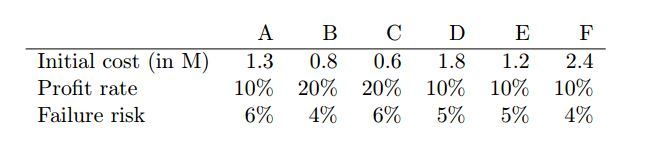
\includegraphics[width=0.7\linewidth]{MErrillLynchExample}
\caption{}
\label{fig:MErrillLynchExample}
\end{figure}

\end{frame}

\begin{frame}
	% - https://www.utdallas.edu/~metin/Or6302/Notes/integer.pdf
\begin{itemize}
\item[a)]Provide a formulation to choose the projects that maximize total expected profit, such that Merrill
Lynch does not invest more than 4M dollars and its average failure risk is not over 5\%. \\ For example,
if Merrill Lynch invests only into A and B, it invests only 2.1M dollars and its average failure risk is
(6\%+4\%)/2=5\%.
\item[b)] Suppose that if A is chosen, B must be chosen. Modify your formulation.
\item[c)] Suppose that if C and D are chosen, E must be chosen. Modify your formulation.
\end{itemize} 
\end{frame}

\begin{frame}
	\frametitle{Branch and Bound}
\begin{framed}
The branch and bound method is a solution approach that partitions the feasible solution space into smaller subsets of solutions
\end{framed}
\end{frame}

\subsection{Depot Location Problem}
\begin{frame}
\frametitle{Depot Location Problem} %DEPOT LOCATION
\end{frame}
%====================================================== %
\subsection{Cutting Plane Algorithm}
%- CUTTING PLANE ALGORITHM FOR PURE INTEGER PROGRAMMING
%- http://www.doc.ic.ac.uk/~br/berc/integerprog.pdf
\begin{frame}
	\frametitle{Cutting Plane Algorithm} 
The rationale behind this approach is :
\begin{itemize}
\item[1.] Solve the continuous problem as an LP i.e. ignore integrality
\item[2.] If by chance the optimal basic variables are all integer then the optimum solution has been found.
Otherwise:
\item[3.] \textbf{Generate a cut} - i.e. a constraint which is satisfied by all integer solutions to the problem but not by the 
current L.P. solution.
\item[4.] Add this new constraint and go to 1 .

\end{itemize}
\end{frame}
%==================================================== %
\subsection{Fathoming}
\begin{frame}
\frametitle{Fathoming}
\Large
	
\end{frame}
%======================================================= %
\subsection{Branch and Bound}
\begin{frame}
	\frametitle{Branch and Bound}
	\Large
	\begin{figure}
\centering
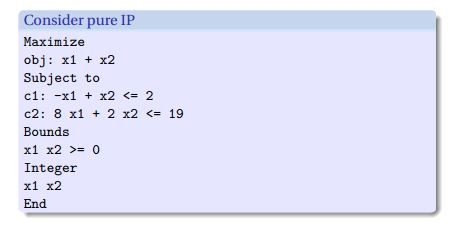
\includegraphics[width=0.7\linewidth]{BranchBound1}
\end{figure}

\end{frame}
\begin{frame}
	\frametitle{Branch and Bound}
	\Large
	\begin{figure}
		\centering
		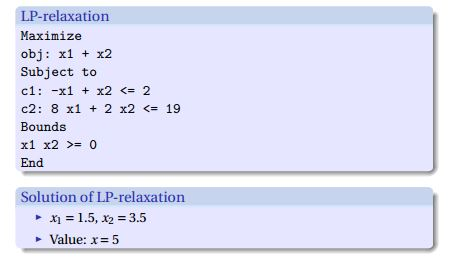
\includegraphics[width=0.7\linewidth]{BranchBound2}
	\end{figure}
	
\end{frame}
\begin{frame}
	\frametitle{Branch and Bound}
	\Large
	\begin{figure}
		\centering
		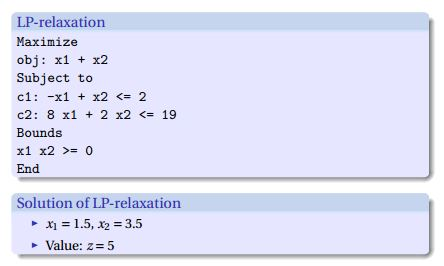
\includegraphics[width=0.7\linewidth]{BranchBound3}
	\end{figure}
	
\end{frame}
\begin{frame}
	\frametitle{Branch and Bound}
	\Large
	\begin{figure}
		\centering
		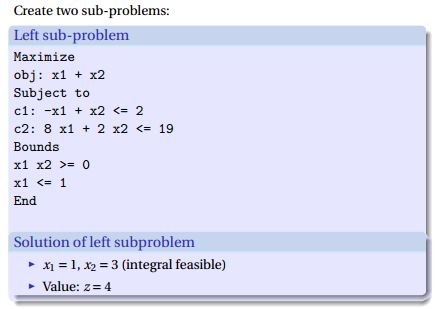
\includegraphics[width=0.7\linewidth]{BranchBound4}
	\end{figure}
	
\end{frame}
\begin{frame}
	\frametitle{Branch and Bound}
	\Large
	\begin{figure}
		\centering
		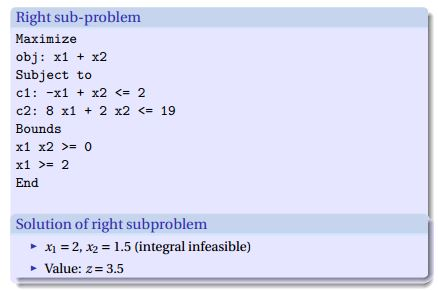
\includegraphics[width=0.7\linewidth]{BranchBound5}
	\end{figure}
	
\end{frame}
\begin{frame}
	\frametitle{Branch and Bound}
	\Large
	\begin{figure}
		\centering
		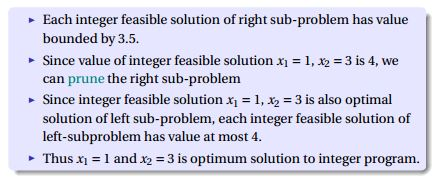
\includegraphics[width=0.7\linewidth]{BranchBound6}
	\end{figure}
	
\end{frame}
\subsection{Difficulties of Integer Programming}
% % - http://www.inf.ufpr.br/aurora/disciplinas/topicosia2/livros/search/integer.pdf
\begin{frame}
	It is not always the case that branch and bound quickly
	solves integer programs. In particular, it is possible that the bounding aspects
	of branch and bound are not invoked, and the branch and bound algorithm can
	then generate a huge number of subproblems. In the worst case, a problem
	with n binary variables (variables that have to take on the value 0 or 1) can
	have $2^n$ subproblems. This exponential growth is inherent in any algorithm for
	integer programming, 
\end{frame}
%======================================================= %
\end{document}
